\documentclass[]{article}

% Imported Packages
%------------------------------------------------------------------------------
\usepackage{amssymb}
\usepackage{amstext}
\usepackage{amsthm}
\usepackage{amsmath}
\usepackage{enumerate}
\usepackage{fancyhdr}
\usepackage[margin=1in]{geometry}
\usepackage{graphicx}
\usepackage{extarrows}
\usepackage{setspace}
%------------------------------------------------------------------------------

% Header and Footer
%------------------------------------------------------------------------------
\pagestyle{plain}  
\renewcommand\headrulewidth{0.4pt}                                      
\renewcommand\footrulewidth{0.4pt}                                    
%------------------------------------------------------------------------------

% Title Details
%------------------------------------------------------------------------------
\title{Deliverable \#3}
\author{Group \#4 \\
Attia, Abrar - attiaa1 - 400017188 \\
Ansell, Evan - ansellea - 1415992 \\
Fayez, Susan - fayezs - 001404420 \\
Yin, Hao - yinh1 - 400016540 \\
Yang, Zhiwen - yangz18 - 400023048 }
\date{2018-03-29}                               
%------------------------------------------------------------------------------
 
% Document
%------------------------------------------------------------------------------
\begin{document}

\maketitle	
\newpage
\section{Introduction}
\label{sec:introduction}
% Begin Section
\subsection{Purpose}
\label{sub:purpose}
% Begin SubSection
 purpose of this document is to provide a more in depth look at the systems within Forester. Specifically, the document goes over the functionality of all classes in the application and how the use cases are completed. The intended audience of this document are mainly the software developers and the project managers. 
% End SubSection

\subsection{System Description}
\label{sub:system_description}
% Begin SubSection

The Forester system is a plant identification system implemented by Blackboard Architecture. It accepts three user types: average users, researchers and administrators. They have different levels of permission to view and manipulate data from the data source. The system stores plant data and identifies designated matches according to the input of users. The users enter a number of different plant characteristics which are checked by the relevant experts. Then the system fetches data from the data source and displays output to the users.
The whole system contains four entities(Plant Data, Search History, Registered Users, Modifications) which hold all the data of the system. With the help of controller classes(I/O Controller, Identification Experts, Security, Modification Controller), users are able to login, edit account information, send input, receive output and edit plant data. The system also consists of eleven boundary classes: Identify Plant, Results, View Search History, Login, Login Error, Change Password, Submit Modifications, Manage Modifications, Researcher and Administrator. They communicate with entity classes by controllers to realize data transmission back and forth.

% End SubSection

\subsection{Overview}
\label{sub:overview}
% Begin SubSection
The remaining sections of this document contains a collection of state charts for the controller classes that exist in the Forester system. Sequence diagrams are then used to display in depth the use cases of the application. Lastly, a detailed class diagram is provided. The document then ends with a division of labour sheet. 

% End SubSection

% End Section
\newpage
\section{State Charts for Controller Classes}
\label{sec:state_charts_for_controller_classes}
% Begin Section
\begin{figure}[!hb]
      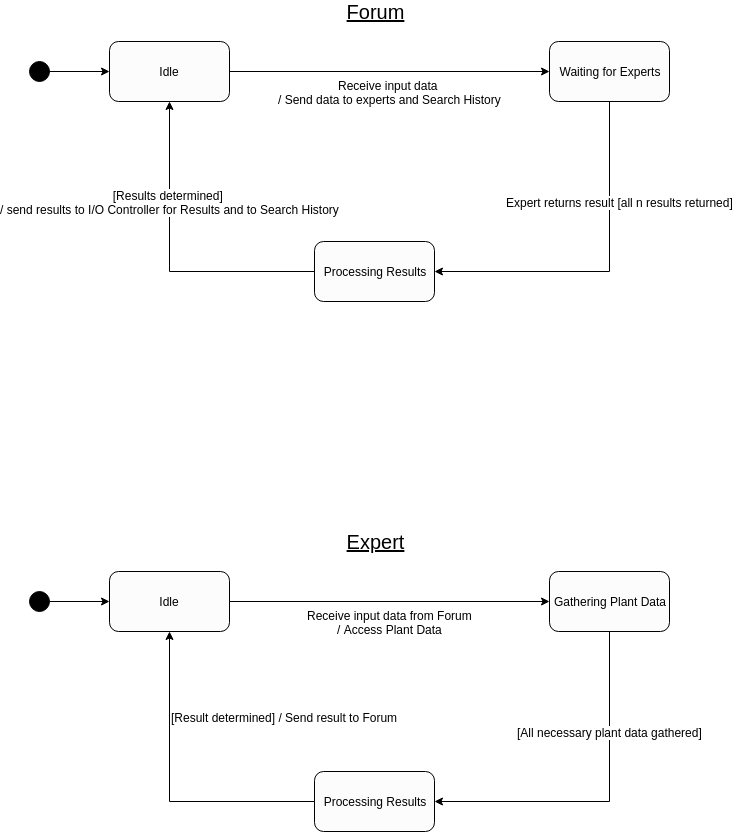
\includegraphics[width=\linewidth]{ForumExpert.png}
      \caption{Forum and Expert State Charts}
      \label{fig:FEState}
\end{figure}

\begin{figure}[!hb]
      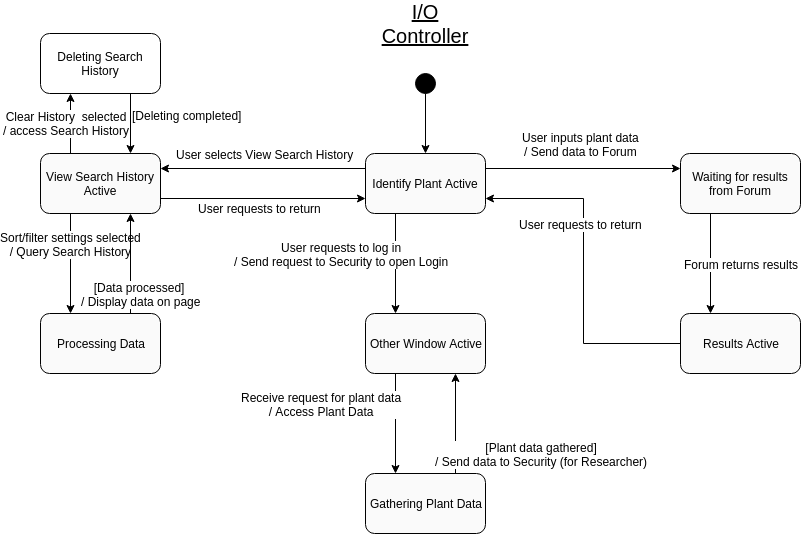
\includegraphics[width=\linewidth]{IOController.png}
      \caption{I/O Controller State Chart}
      \label{fig:IOState}
\end{figure}

\begin{figure}[!hb]
      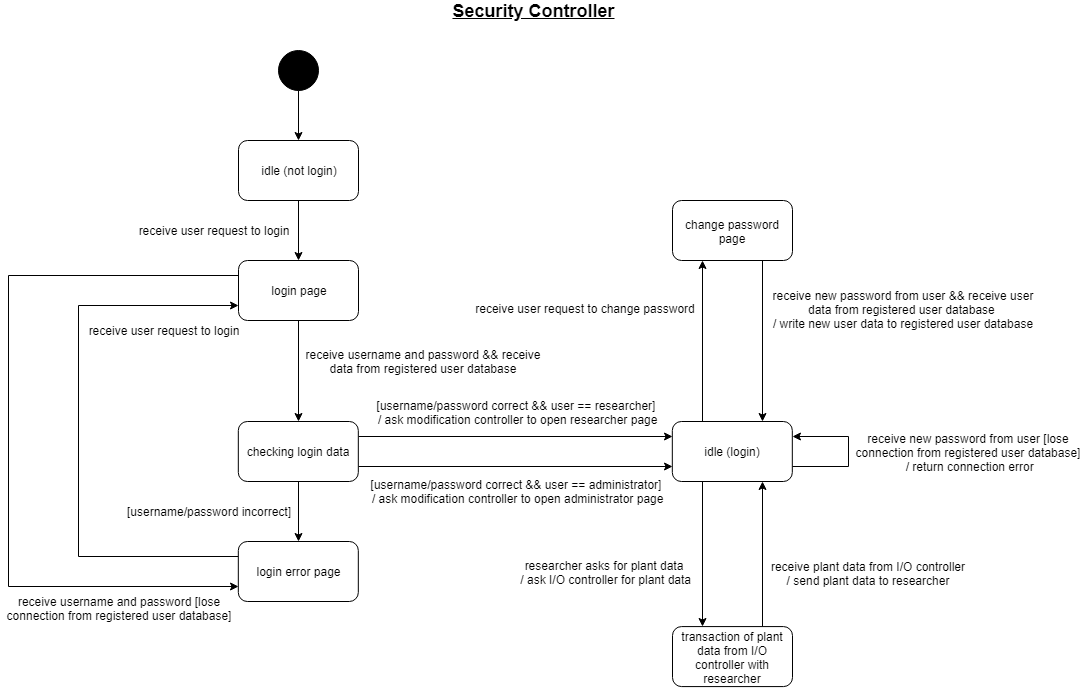
\includegraphics[width=\linewidth]{SecurityController.png}
      \caption{Security Controller State Chart}
      \label{fig:SCState}
\end{figure}

\begin{figure}[!hb]
      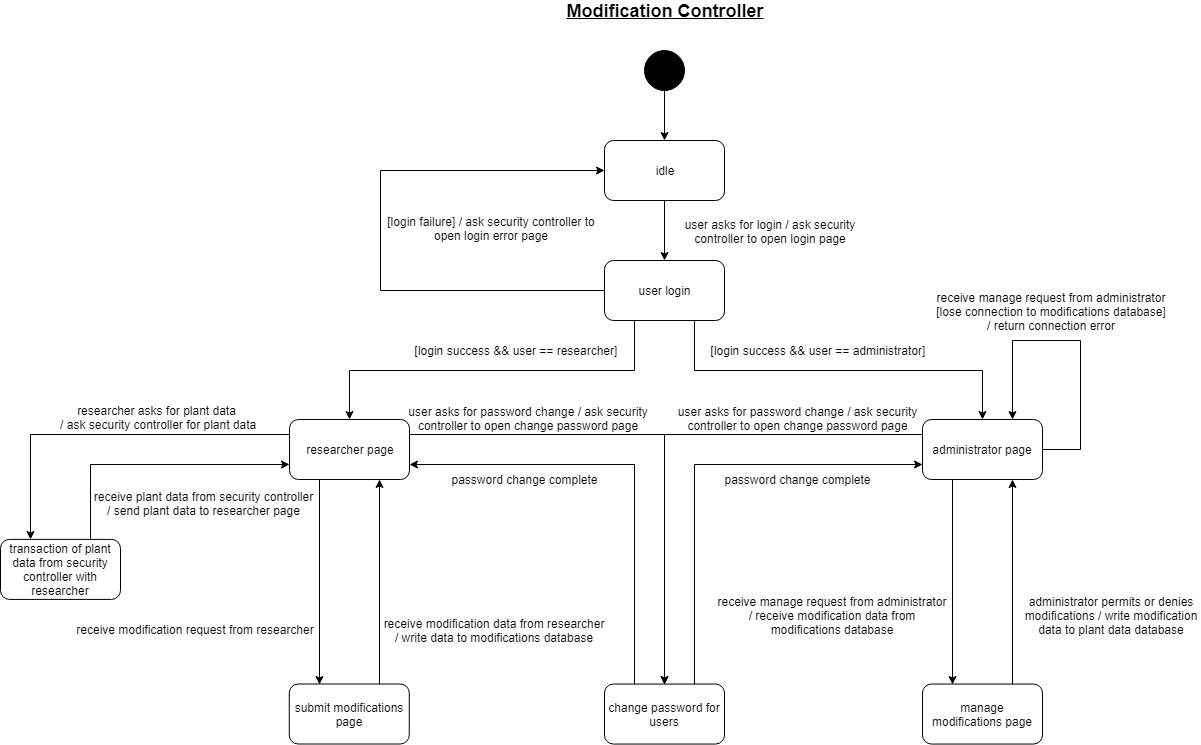
\includegraphics[width=\linewidth]{ModificationController.png}
      \caption{Modification Controller State Chart}
      \label{fig:MCState}
\end{figure}
    
% End Section
\clearpage

\section{Sequence Diagrams}
\label{sec:sequence_diagrams}
% Begin Section
\begin{figure}[h!]
\centering
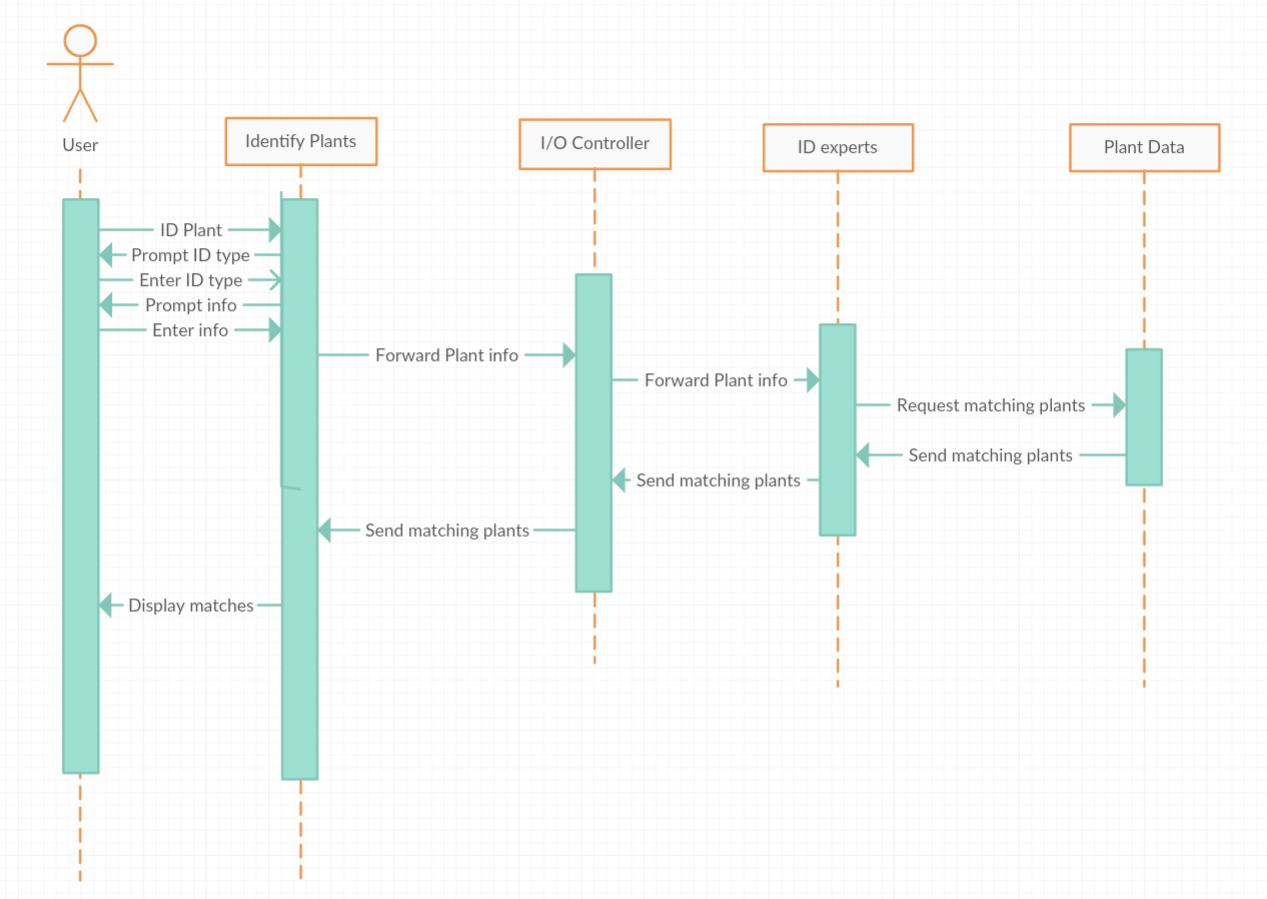
\includegraphics[scale=0.6]{IdentifyPlants.png}
\caption{Identify Plants}
\label{fig:s1}
\end{figure}

\begin{figure}[h!]
\centering
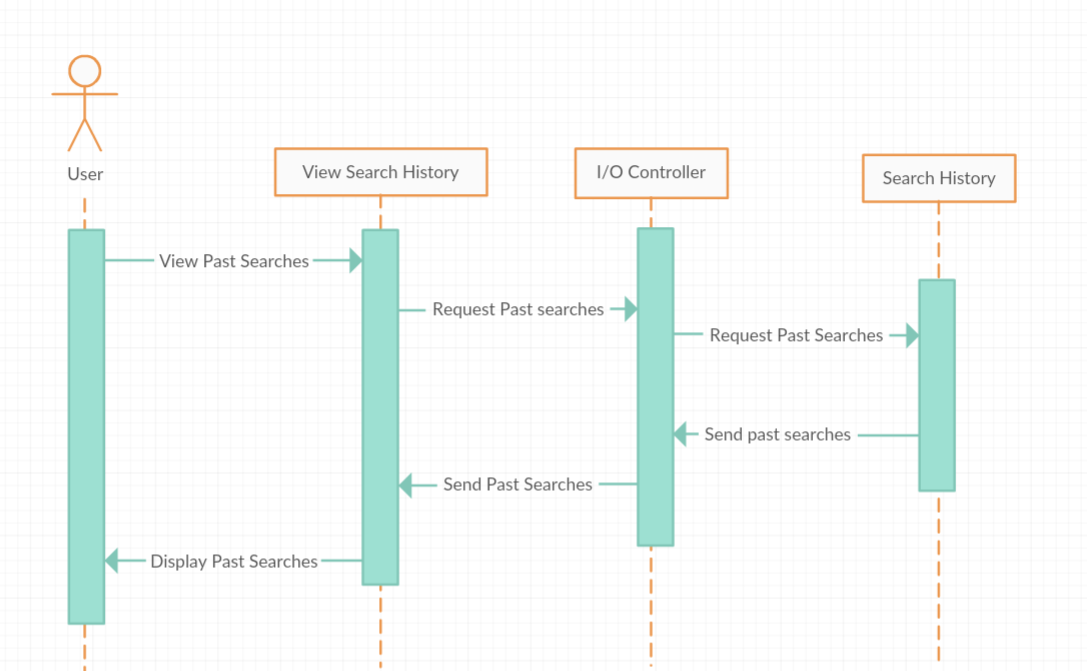
\includegraphics[scale=0.6]{ViewPastSearches.png}
\caption{View Past Searches}
\label{fig:s2}
\end{figure}

\begin{figure}[h!]
\centering
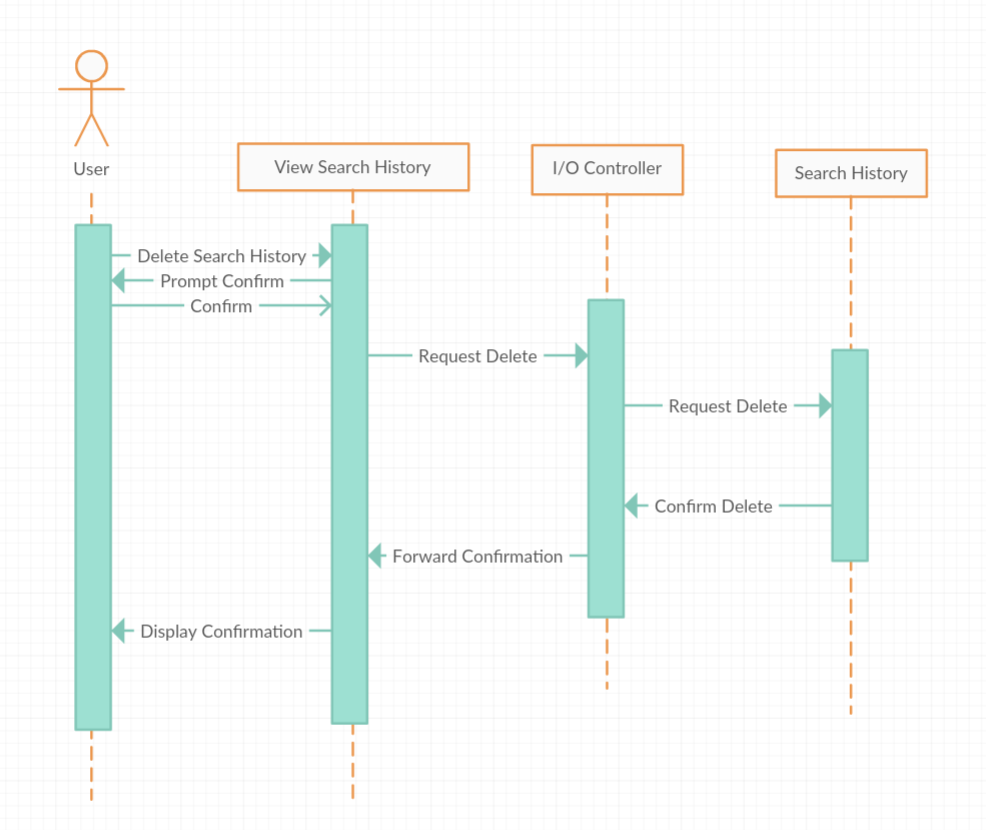
\includegraphics[scale=0.6]{DeleteSearchHistory.png}
\caption{Delete Search History}
\label{fig:s3}
\end{figure}

\begin{figure}[h!]
\centering
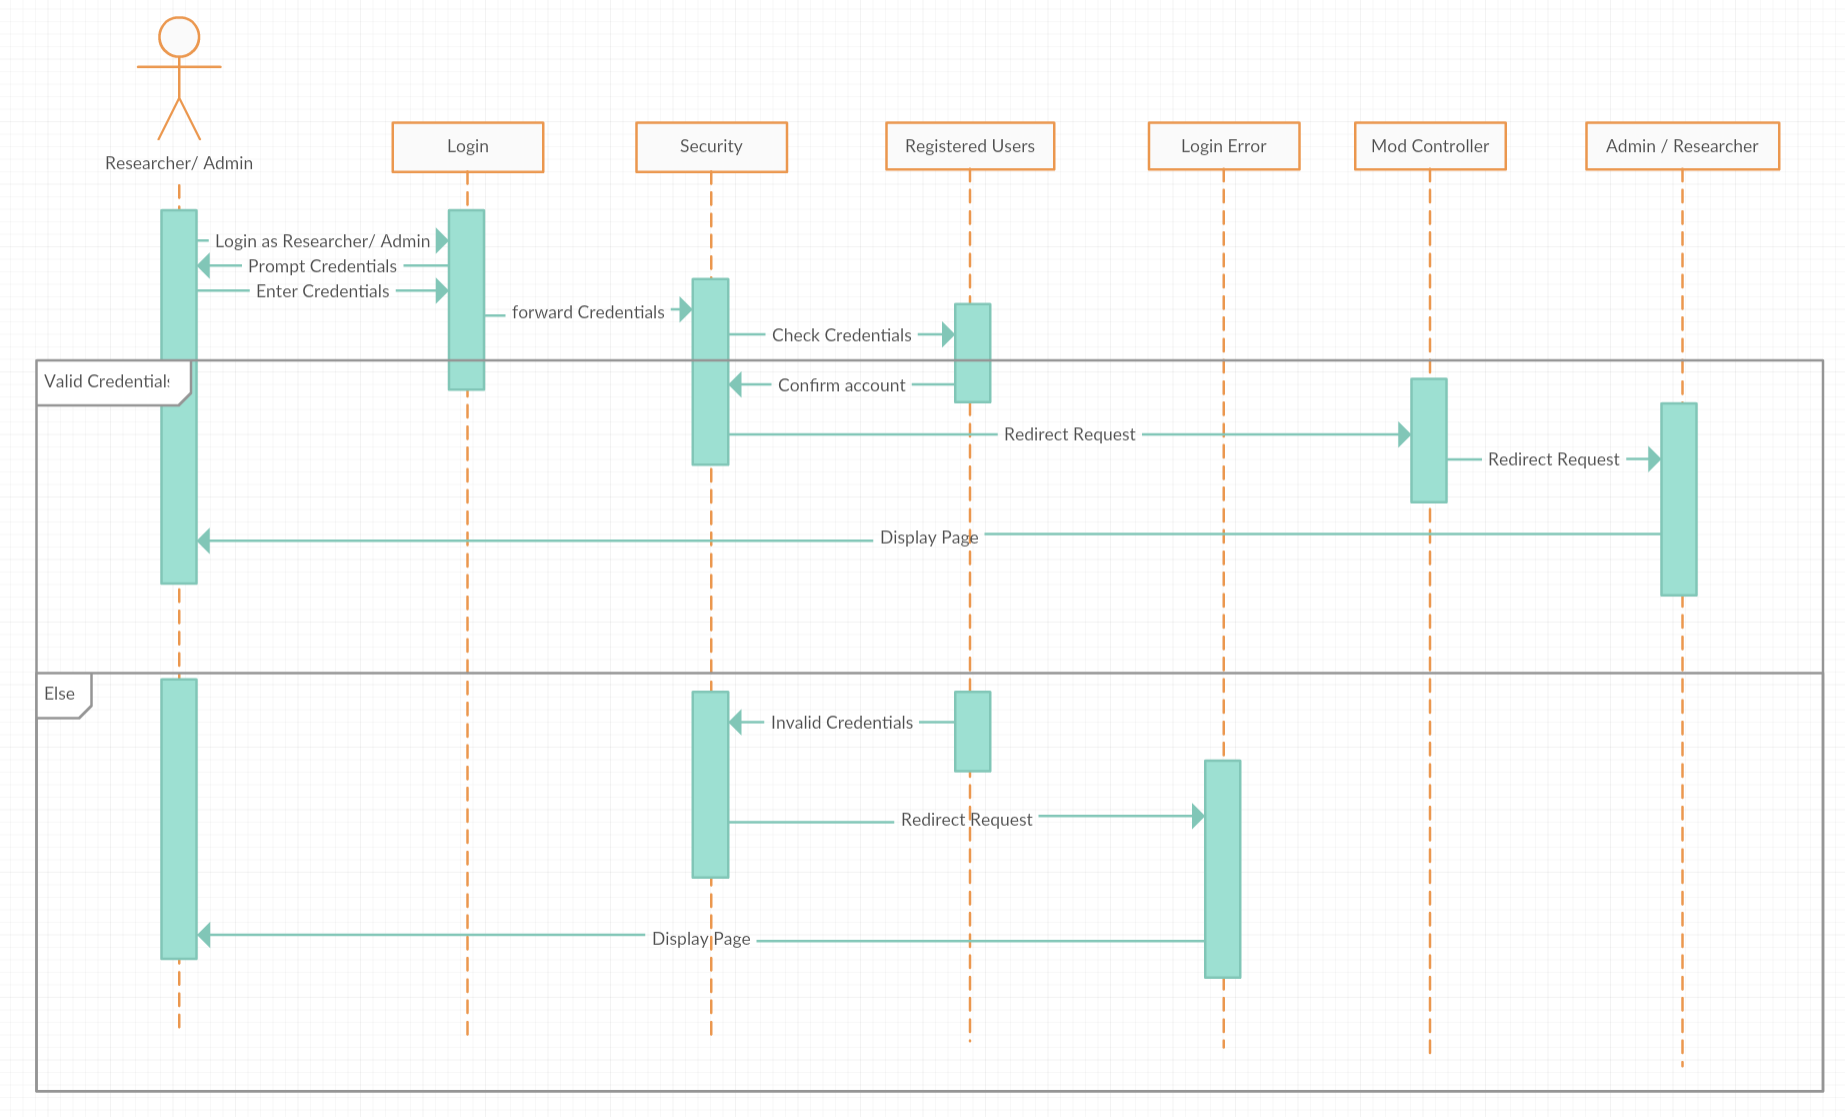
\includegraphics[scale=0.42]{Login.png}
\caption{Login}
\label{fig:s4}
\end{figure}

\begin{figure}[h!]
\centering
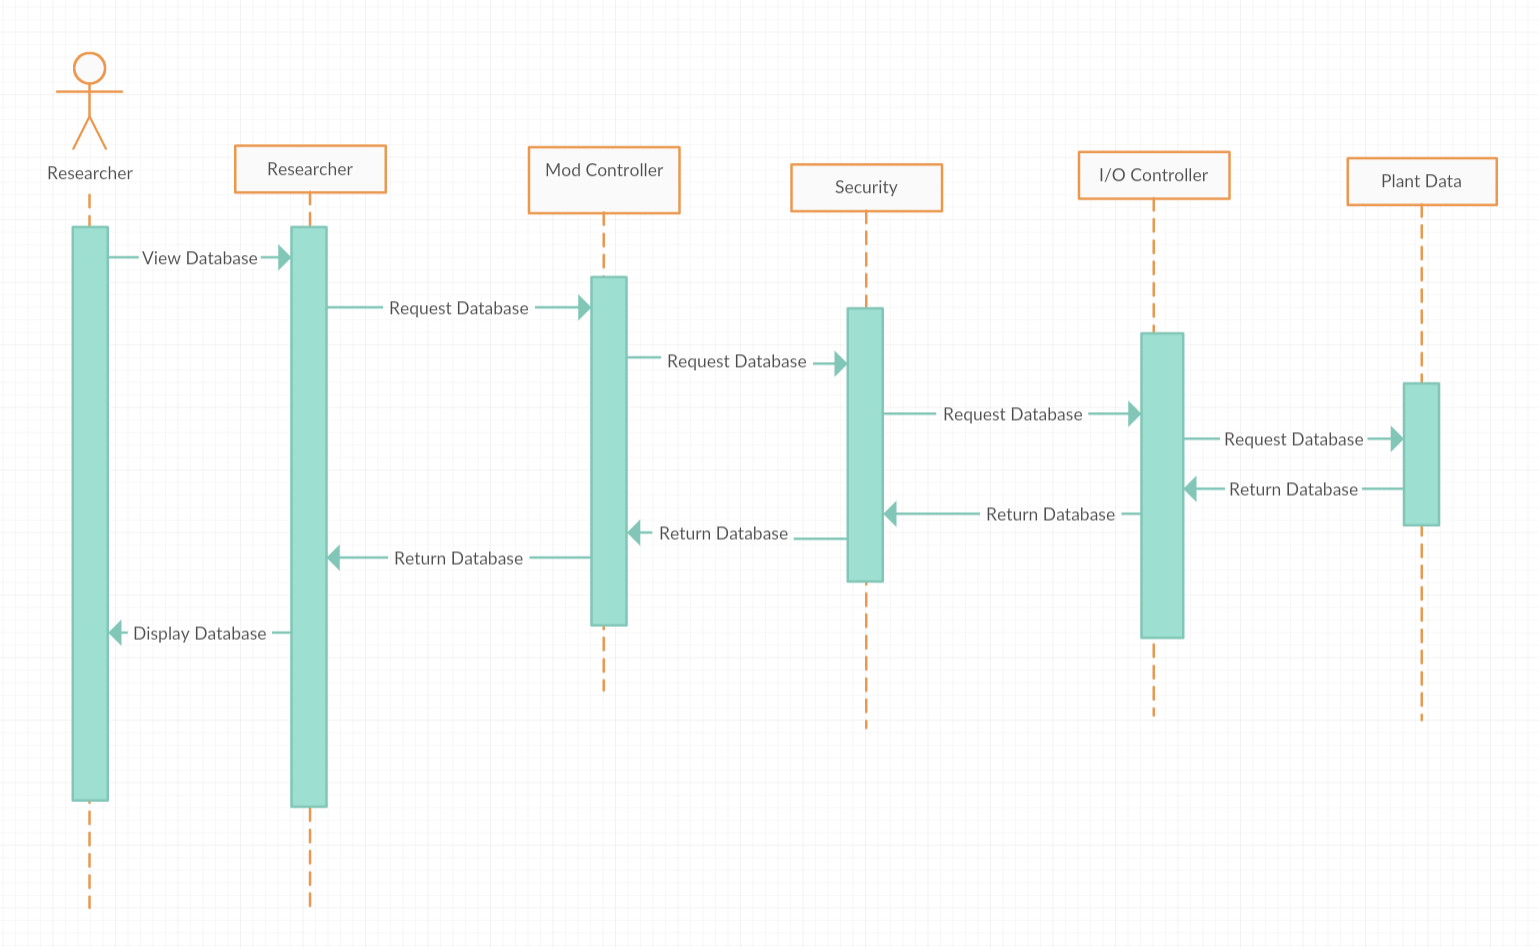
\includegraphics[scale=0.48]{viewdatabase.png}
\caption{View Database}
\label{fig:s5}
\end{figure}

\begin{figure}[h!]
\centering
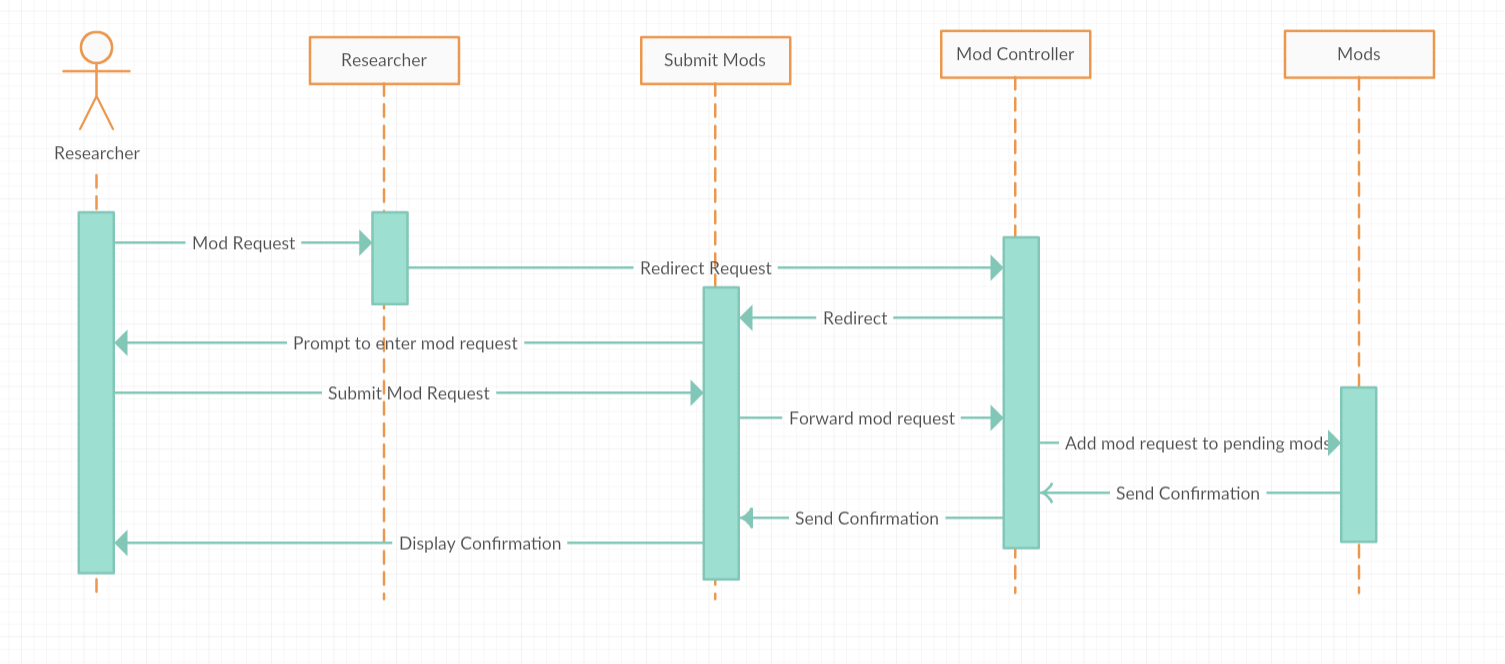
\includegraphics[scale=0.51]{SubmitRequests.png}
\caption{Submit Requests}
\label{fig:s6}
\end{figure}

\begin{figure}[h!]
\centering
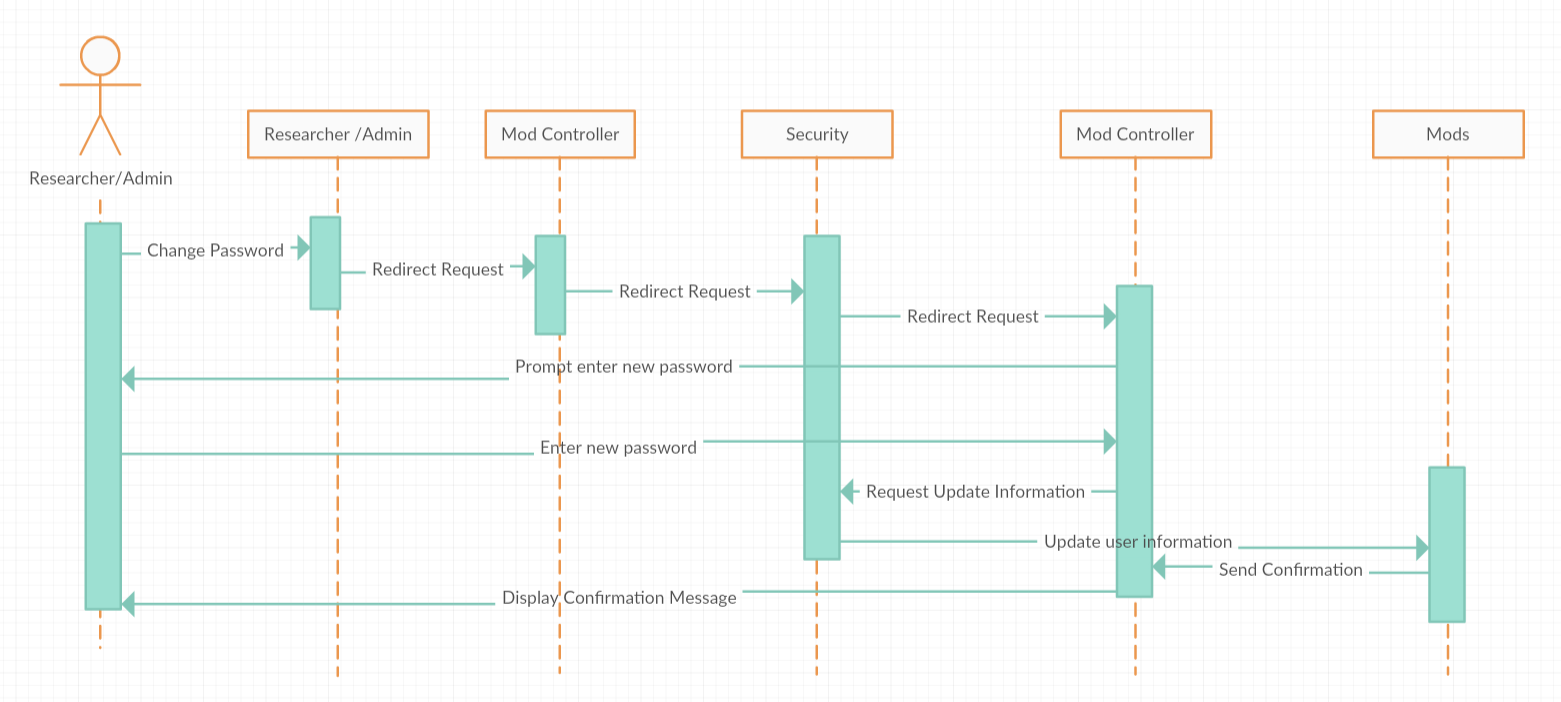
\includegraphics[scale=0.5]{updatepassword.png}
\caption{Update Password}
\label{fig:s7}
\end{figure}

\begin{figure}[h!]
\centering
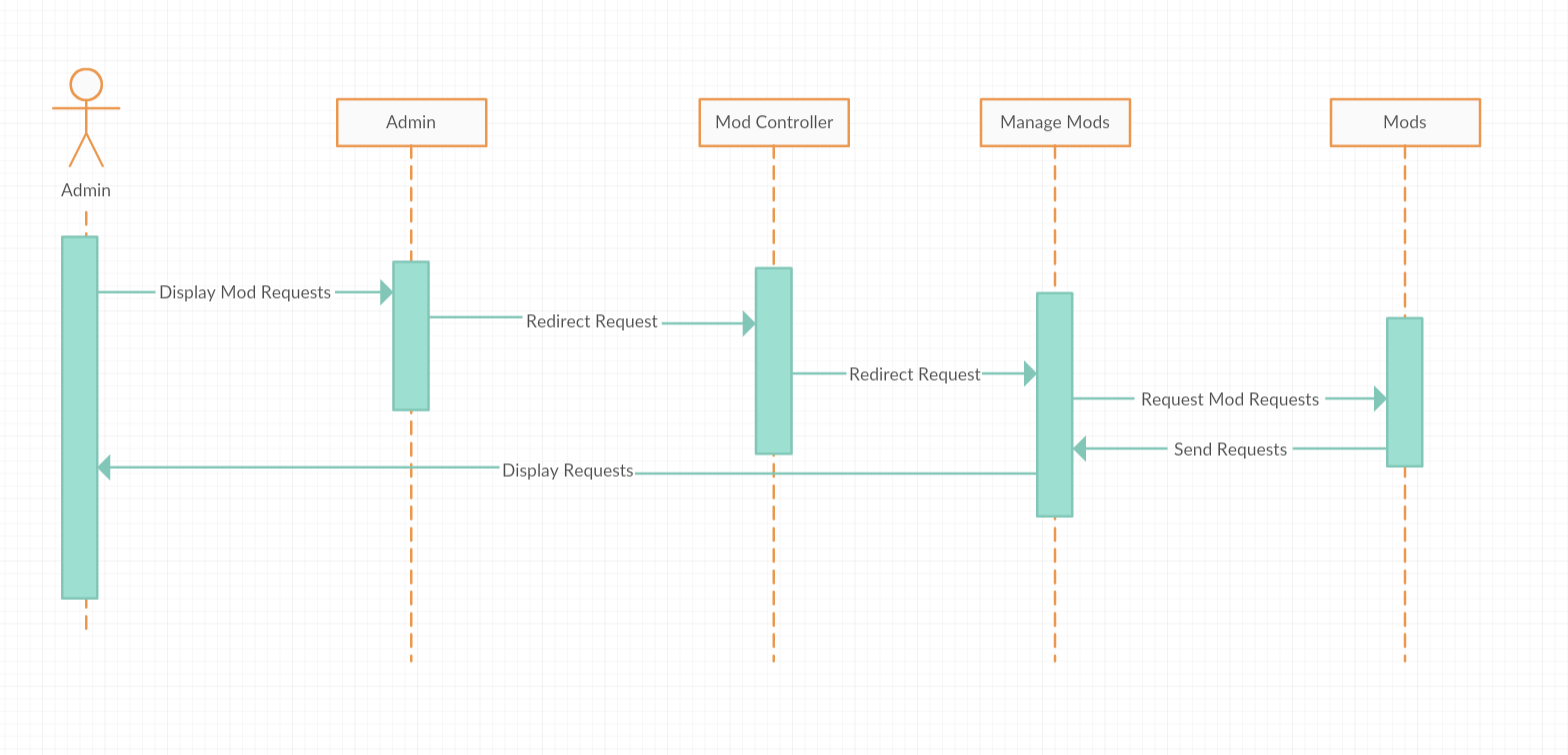
\includegraphics[scale=0.5]{displayrequest.png}
\caption{Display Requests}
\label{fig:s8}
\end{figure}

\begin{figure}[h!]
\centering
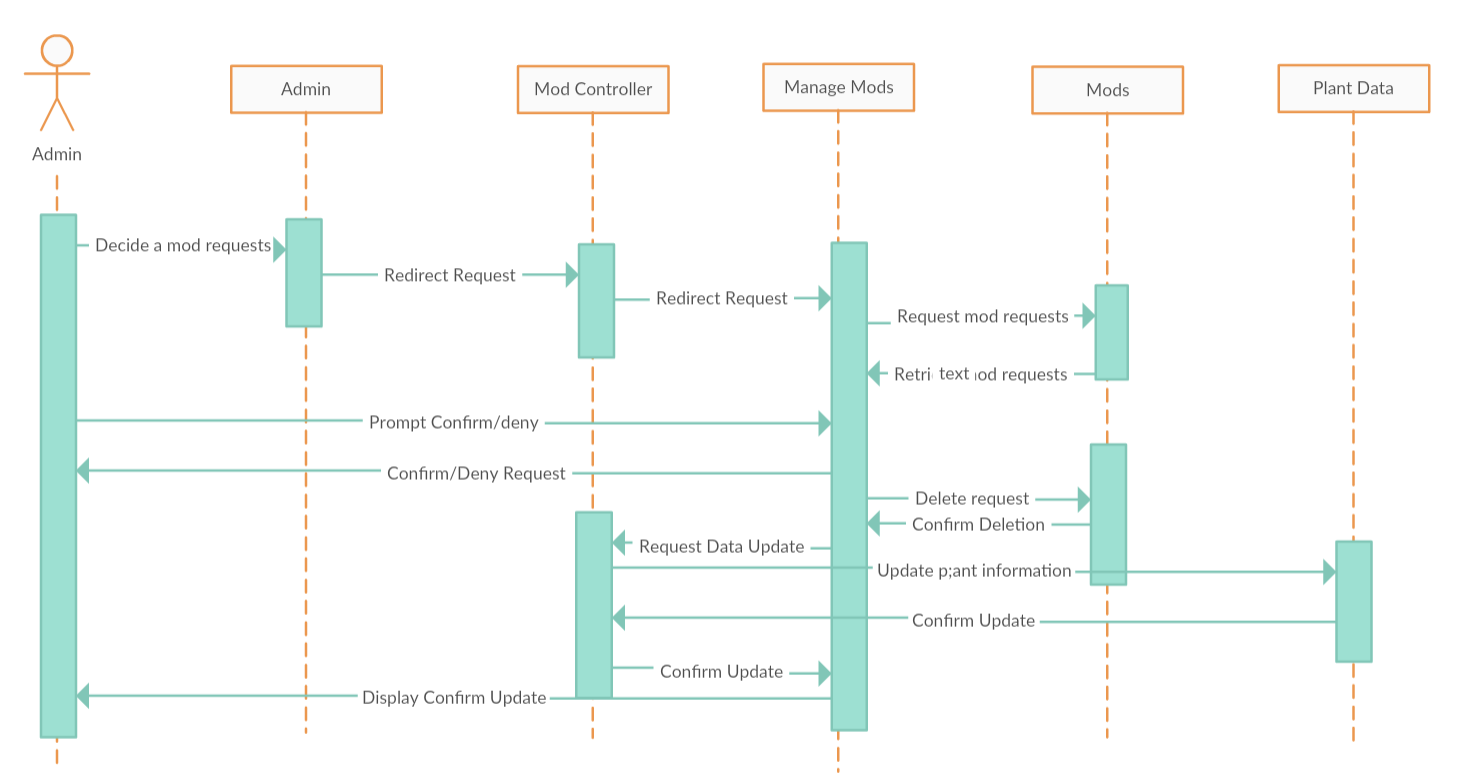
\includegraphics[scale=0.5]{Decideanrequests.png}
\caption{Decide mod requests}
\label{fig:s9}
\end{figure}
\clearpage
% End Section

\section{Detailed Class Diagram}
\label{sec:detailed_class_diagram}
% Begin Section
Note: The Detailed Class Diagram is divided into 2 sections in order to allow for more clarity. The placeholder (S2) connects both sections of the diagram together. 
\begin{figure}[!hb]
      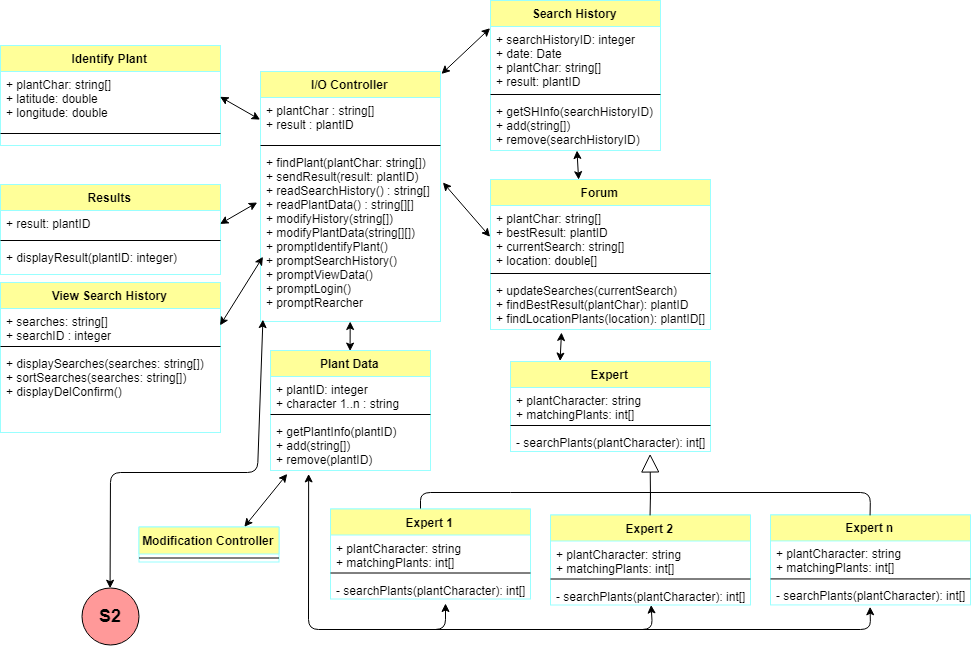
\includegraphics[width=\linewidth]{ClassDiagramP1.png}
      \caption{Detailed Class Diagram - Top Half}
      \label{fig:CD1}
\end{figure}
\begin{figure}[!hb]
      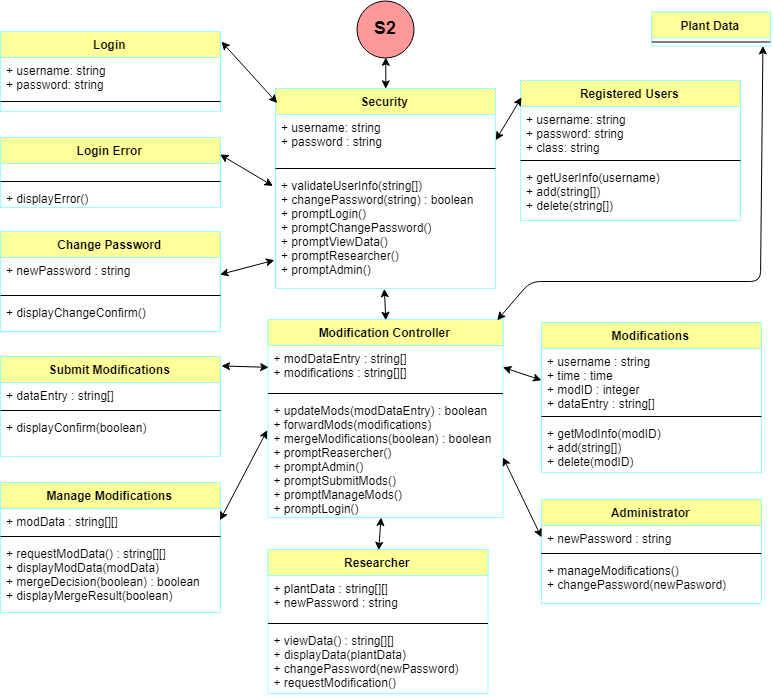
\includegraphics[width=\linewidth]{ClassDiagramP2.png}
      \caption{Detailed Class Diagram - Bottom Half}
      \label{fig:CD2}
\end{figure}
% End Section
\clearpage

\end{document}
%------------------------------------------------------------------------------
